\chapter{Implementation on an edge device and validation in a real environment}
\label{cap:edge}

In Chapter~\ref{cap:sperimentale} the system was evaluated on recordings already available, without imposing any constraint on the time needed to process each frame. In this chapter we shall instead verify the operation of the whole pipeline, analysing the porting to a Radxa ROCK 4D, the computational cost and the choice of the operating configuration. We shall then move to a real environment and analyse the domestic acquisitions, evaluating the system during prolonged operation and in the passage from metrics on the individual windows to alarm events.

\section{Edge platform and operating configuration}
\label{sec:piattaforma}

A \textbf{Radxa ROCK 4D} with a Rockchip RK3576 SoC, 6~GB of memory and an integrated 6~TOPS NPU was used for the implementation. The overall cost of the platform, USB camera included, is of the order of a hundred euros per acquisition point.
Unlike a centralised architecture, in which one or more cameras send the images to an external server, here the whole pipeline is executed locally: acquisition, pose estimation, feature extraction and classification. Only the information associated with a possible alarm is transmitted outside.

\begin{table}[htbp]
\centering
\caption{Comparison between local processing on an edge device and the use of a remote server.}
\label{tab:edge_vs_server}
\begin{tabularx}{\textwidth}{@{}lXX@{}}
\toprule
& \textbf{Edge node} & \textbf{Server with GPU} \\
\midrule
Computation & ARM SoC + NPU & x86 CPU + dedicated GPU \\
Cost & per node & shared infrastructure \\
Network required & not necessary & necessary \\
Data transmitted & alarm information & video stream \\
\bottomrule
\end{tabularx}
\end{table}

The main difference concerns the \textbf{cost per room}. A server can be shared between several cameras, but requires each of them to transmit its own video stream continuously. This reduces the computational cost per individual room, but increases the dependence on the network and the data have to leave the home. An edge node dedicated to each room does not enjoy the same economy of scale, but has a known cost per installation and keeps the processing and the data local, as required in Chapter~\ref{cap:contesto}.

\subsection{Porting constraints}

Three main problems emerged during the porting.

The first concerns the architecture of the processor. The more recent versions of MediaPipe tried on the board are compiled for ARMv8.1, whereas the RK3576 implements ARMv8.0. Execution terminated with an \texttt{illegal instruction} error. Version 0.10.9 works correctly and was therefore retained.

The second problem concerns the interface used by the code. The more recent versions of MediaPipe have progressively replaced the \texttt{mp.solutions} interface, on which the feature extraction pipeline had been built. Changing interface would have required modifying a significant part of the code already used in the earlier experiments. This too is a reason why the version compatible with the existing pipeline was retained.

The third problem emerged during the trials with the NPU. The converted model requires a four-dimensional input tensor. With a three-dimensional tensor the inference was not executed, but no explicit error was returned. The time measured therefore came out very low without the model having actually processed the data. From this trial onwards it was verified that the computation was really being carried out and that the output was correct before any speed measurement was used.

\section{Verification of equivalence between computer and device}
\label{sec:parita}

Before measuring performance on the board, it was verified that the classifier produced the same results as those obtained on the computer.
The first trial was carried out on 200 windows already computed, thereby excluding the camera and the pose estimator.

\begin{table}[htbp]
\centering
\caption{Comparison of the predictions on 200 precomputed windows.}
\label{tab:parita}
\begin{tabular}{lr}
\toprule
Maximum discrepancy between the predictions & $2{,}2\times10^{-16}$ \\
Differing decisions & 0 \\
\bottomrule
\end{tabular}
\end{table}

No differing decisions were observed. At parity of features, normalisation and classifier, the two systems therefore produce the same result. The comparison was then repeated starting directly from the videos. Out of 56 clips, 55 produced the same final decision. In one recording alone, containing a fall, the decision turned out different.
The difference arises before the classifier. MediaPipe maintains a temporal state in order to follow the person, and small variations in the landmarks change the features obtained. When the score is close to the threshold, this variation can change the final decision.

Some faulty measurements were identified during these tests. In one trial different models showed almost identical times because no person was detected in the frames used. In another trial about 1.315~fps were measured because the inference on the NPU was not being executed, owing to the wrong input shape.
An early check on the landmarks was also too weak: it verified only that the coordinates were positive, and therefore treated as valid even points that were clearly placed wrongly. The measurements reported in the following sections are therefore used only after both the execution of the computation and the consistency of the output have been checked.

\subsection{Comparison between pose estimators}
\label{sec:stimatore}

Pose estimation is the most expensive stage of the pipeline. MediaPipe on the CPU of the Radxa takes about 92,6~ms per frame, that is 10,8~fps. It is therefore not possible to keep the 18~fps of the original dataset. In order to increase the speed, YOLOv8-pose quantised to INT8 and run on the NPU was tried.

The inference alone turns out to be 5,16 times faster. The gain for the whole pipeline was initially 1,71 times, because the post-processing took 12,14~ms per frame. After this part of the code had been vectorised, the time dropped to 0,94~ms and the overall gain rose to 2,17 times.
Speed alone is not, however, enough. The quality of the pose was therefore verified over 29.681 frames belonging to different activities.

\begin{table}[htbp]
\centering
\caption{Pose retention with YOLOv8-pose INT8 and MediaPipe. Five-subject experiment.} \label{tab:ritenzione}
\begin{tabular}{lcc}
\toprule
\textbf{Activity} & \textbf{YOLOv8 INT8} & \textbf{MediaPipe} \\
\midrule Standing, sitting down, picking up, jumping & 100\% & 100\% \\
Forward fall onto the hands & 79,2\% & 99,5\% \\
\textbf{Lying down} & \textbf{43,6\%} & \textbf{79,1\%} \\
\bottomrule
\end{tabular}
\end{table}

The difference appears above all when the person is close to the floor. For the lying position, YOLOv8 keeps the detection in 43,6\% of the frames against 79,1\% for MediaPipe. Lowering the YOLOv8 threshold to 0,05 brings it to 58,9\%, still below MediaPipe.

A difference in the estimated geometry was also observed. With YOLOv8 the projected length of the torso goes from 83,5 pixels when standing to 56,5 pixels on the ground. With MediaPipe it goes instead from 83,8 to 100,7 pixels. This quantity is used in the body-centric normalisation. An error in the length of the torso therefore changes several features at once. In order to measure the final effect, the two estimators were compared while features, classifier, threshold and protocol were kept unchanged.

\begin{table}[H]
\centering
\caption{Performance obtained by replacing the pose estimator. Five-subject experiment.}
\label{tab:stimatori_f2}
\begin{tabular}{lccc}
\toprule
\textbf{Estimator} & \textbf{$F_2$} & \textbf{FP} & \textbf{FN} \\
\midrule MediaPipe & $0{,}909 \pm 0{,}095$ & 17 & 23 \\
YOLOv8 INT8 & $0{,}682 \pm 0{,}044$ & 225 & 59 \\
\bottomrule
\end{tabular}
\end{table}

The mean difference of $F_2$ is 0,227, and YOLOv8 increases both the false positives and the false negatives. These values come from the five-subject experimental configuration and were not repeated after the extension to ten subjects. They are therefore used as indicative results for the choice of the estimator, whereas the timing measurements were obtained directly on the board.

\subsection{Choice of the operating configuration}
\label{sec:decisione}

The final choice must hold together processing frequency and quality of the pose. The Random Forest was used on the board. In the tests of Chapter~\ref{cap:sperimentale} some neural networks obtain slightly better results, but the differences between the main architectures remain small with respect to the variability observed between subjects. The Random Forest was therefore preferred because it is simpler to run on the device, does not require the TensorFlow stack and reduces the software dependencies of the pipeline.

\begin{table}[htbp]
\centering
\caption{Configurations considered for operation on the device.}
\label{tab:catene}
\begin{tabular}{llccc}
\toprule \textbf{Configuration} & \textbf{On the device} & \textbf{$F_2$} & \textbf{FP} & \textbf{FN} \\
\midrule
MediaPipe @ 18 fps & not attainable & 0,898 & 23 & 24 \\
MediaPipe @ 9 fps & 10,8 fps & 0,857 & 57 & 49 \\
YOLOv8 @ 18 fps & 26,5 fps & 0,682 & 225 & 59 \\
\bottomrule
\end{tabular}
\end{table}

MediaPipe at 18~fps is not usable on the board, but it reaches 10,8~fps and can therefore be used with a sequence subsampled to 9 samples per second. Moreover, of the two configurations that can actually be run, MediaPipe at 9~fps keeps the better results: $F_2=0{,}857$ against 0,682 for YOLOv8, while recall is 0,866 and 0,775 respectively. The number of errors is lower as well: 49 false negatives and 57 false positives with MediaPipe, against 59 and 225 with YOLOv8.

\begin{table}[htbp]
\centering
\caption{Variation of $F_2$ associated with subsampling and with the change of pose estimator.}
\label{tab:scomposizione}
\begin{tabular}{lr}
\toprule
\textbf{Change} & \textbf{$\Delta F_2$} \\
\midrule MediaPipe from 18 to 9 fps & $-0{,}041$ \\
MediaPipe $\rightarrow$ YOLOv8 INT8 & $-0{,}216$ \\
\midrule Ratio between the variations & $5{,}3\times$ \\
\bottomrule
\end{tabular}
\end{table}

In the comparison carried out, changing estimator costs about five times more than halving the frequency. MediaPipe was therefore retained, and the model intended for the board was trained at 9 samples per second.
Subsampling does nonetheless have a cost, reported in Table~\ref{tab:catene}: the false negatives go from 24 to 49 and $F_2$ drops by $0{,}041$. YOLOv8 was evaluated only in the INT8 version. It is therefore not possible to separate the effect of the network from that of the quantisation.

The NPU remains useful from a computational point of view: the inference of YOLOv8-pose is 5,16 times faster and, after the post-processing has been optimised, the pipeline reaches 26,5~fps. The limitation observed in this trial therefore concerns the quality of the estimator used, not the capability of the accelerator.

\section{Computational performance and continuity of operation}

Once the configuration had been chosen, the cost of the various stages and the behaviour of the board during prolonged trials were measured.

\subsection{Computational cost and processing frequency}
\label{sec:costo-computazionale}

In order to assess the computational cost, two cases were considered separately: the accelerated chain with YOLOv8-pose on the NPU, shown in Table~\ref{tab:costo}, and the configuration actually installed, based on MediaPipe on the CPU.

\begin{table}[htbp]
\centering
\caption{Cost per frame of the accelerated chain with YOLOv8-pose on the NPU.}
\label{tab:costo}
\begin{tabular}{lrr}
\toprule
\textbf{Stage} & \textbf{Time} & \textbf{Share} \\
\midrule
Pre-processing & 1,21 ms & 3,2\% \\
Perception & 33,34 ms & 88,4\% \\
Post-processing & 0,94 ms & 2,5\% \\
Classification, amortised cost & 2,21 ms & 5,9\% \\
\midrule
Total & 37,7 ms & 100\% \\
\bottomrule
\end{tabular}
\end{table}

The overall time is about 37,7~ms per frame, corresponding to 26,5~fps. This configuration is not, however, the one used in the domestic trials. The figure does show that the dominant stage remains pose estimation, which takes up 88,4\% of the total time. The values for the accelerated chain come from a dedicated benchmark and were initially transcribed from the terminal. The measurement was not subsequently repeated with the same automatic instrumentation used for the installed chain. This constitutes a limitation on the reproducibility of the measurement.

The configuration actually installed uses MediaPipe on the CPU instead. The times were measured directly on the board during the continuous session of 6 September, lasting 4,59~hours, and are reported in Table~\ref{tab:costo_installato}.

\begin{table}[htbp]
\centering
\caption{Cost per frame of the installed configuration.}
\label{tab:costo_installato}
\begin{tabularx}{\textwidth}{Xrrr}
\toprule
\textbf{Stage} & \textbf{Time} & \textbf{Share} & \textbf{Accelerated chain} \\
\midrule
Perception & 116,38 ms & 85,2\% & 33,34 ms \\
Classification, amortised cost & 19,51 ms & 14,3\% & 2,21 ms \\
Other operations & 0,76 ms & 0,6\% & 2,15 ms \\
\midrule
Total & 136,65 ms & 100\% & 37,7 ms \\
Frequency & 7,3 fps & & 26,5 fps \\
\bottomrule
\end{tabularx}

\end{table}

On the board the Random Forest takes 39,04~ms to classify a window. Since one decision is produced every two frames, the mean cost is 19,51~ms per frame. The remaining 0,76~ms cover the operations not included in the perception and classification measurements, such as frame acquisition, format conversion, buffer updating and data logging.

For the accelerated chain the item ``other operations'' instead collects pre-processing and post-processing, amounting to $1{,}21+0{,}94=2{,}15$~ms.
In both configurations the bottleneck remains perception: 88,4\% of the time in the accelerated chain and 85,2\% in the installed one. Changing the classifier would therefore have a limited effect on the overall frequency.

The mean time of 136,65~ms corresponds to about 7,3~fps. The real frequency is not, however, constant: across the twelve domestic sessions it ranges between 1,15 and 8,20~fps, while in the two prolonged trials it is 7,26 and 6,47~fps. This variability also changes the temporal duration of the windows. The 22 samples used by the classifier correspond to 2,44~s at the design frequency of 9~fps, but to about 3,40~s when the frequency drops to 6,47~fps. During execution the same window may therefore represent a longer time interval than the one used during training.

\subsection{Thermal stability and prolonged operation}
\label{sec:continuita}

Besides processing speed, the ability of the
device to operate continuously without an evident reduction in performance due to temperature was verified. A first ten-minute trial was carried out, for a total of 18.291 inferences.
The variation in latency between the beginning and the end was 3,9\%. The frequency of the accelerator remained at 950~MHz and the temperature settled between 60 and 63~$^\circ$C.

A second check was obtained during the prolonged domestic session of 11 August, which lasted 6,11~hours of wall clock. This session is used here for the thermal measurement alone, and is not the reference continuous trial: the operating system suspended it for about 68 minutes, so that the effective operating time was 4,99~hours, and the dual-clock check that makes such an interruption detectable was introduced only afterwards. The maximum temperature recorded was 79,5~$^\circ$C and it settled after about forty minutes. No sudden drops in the frame rate attributable to \emph{thermal throttling} were observed.

\begin{figure}[H]
\centering
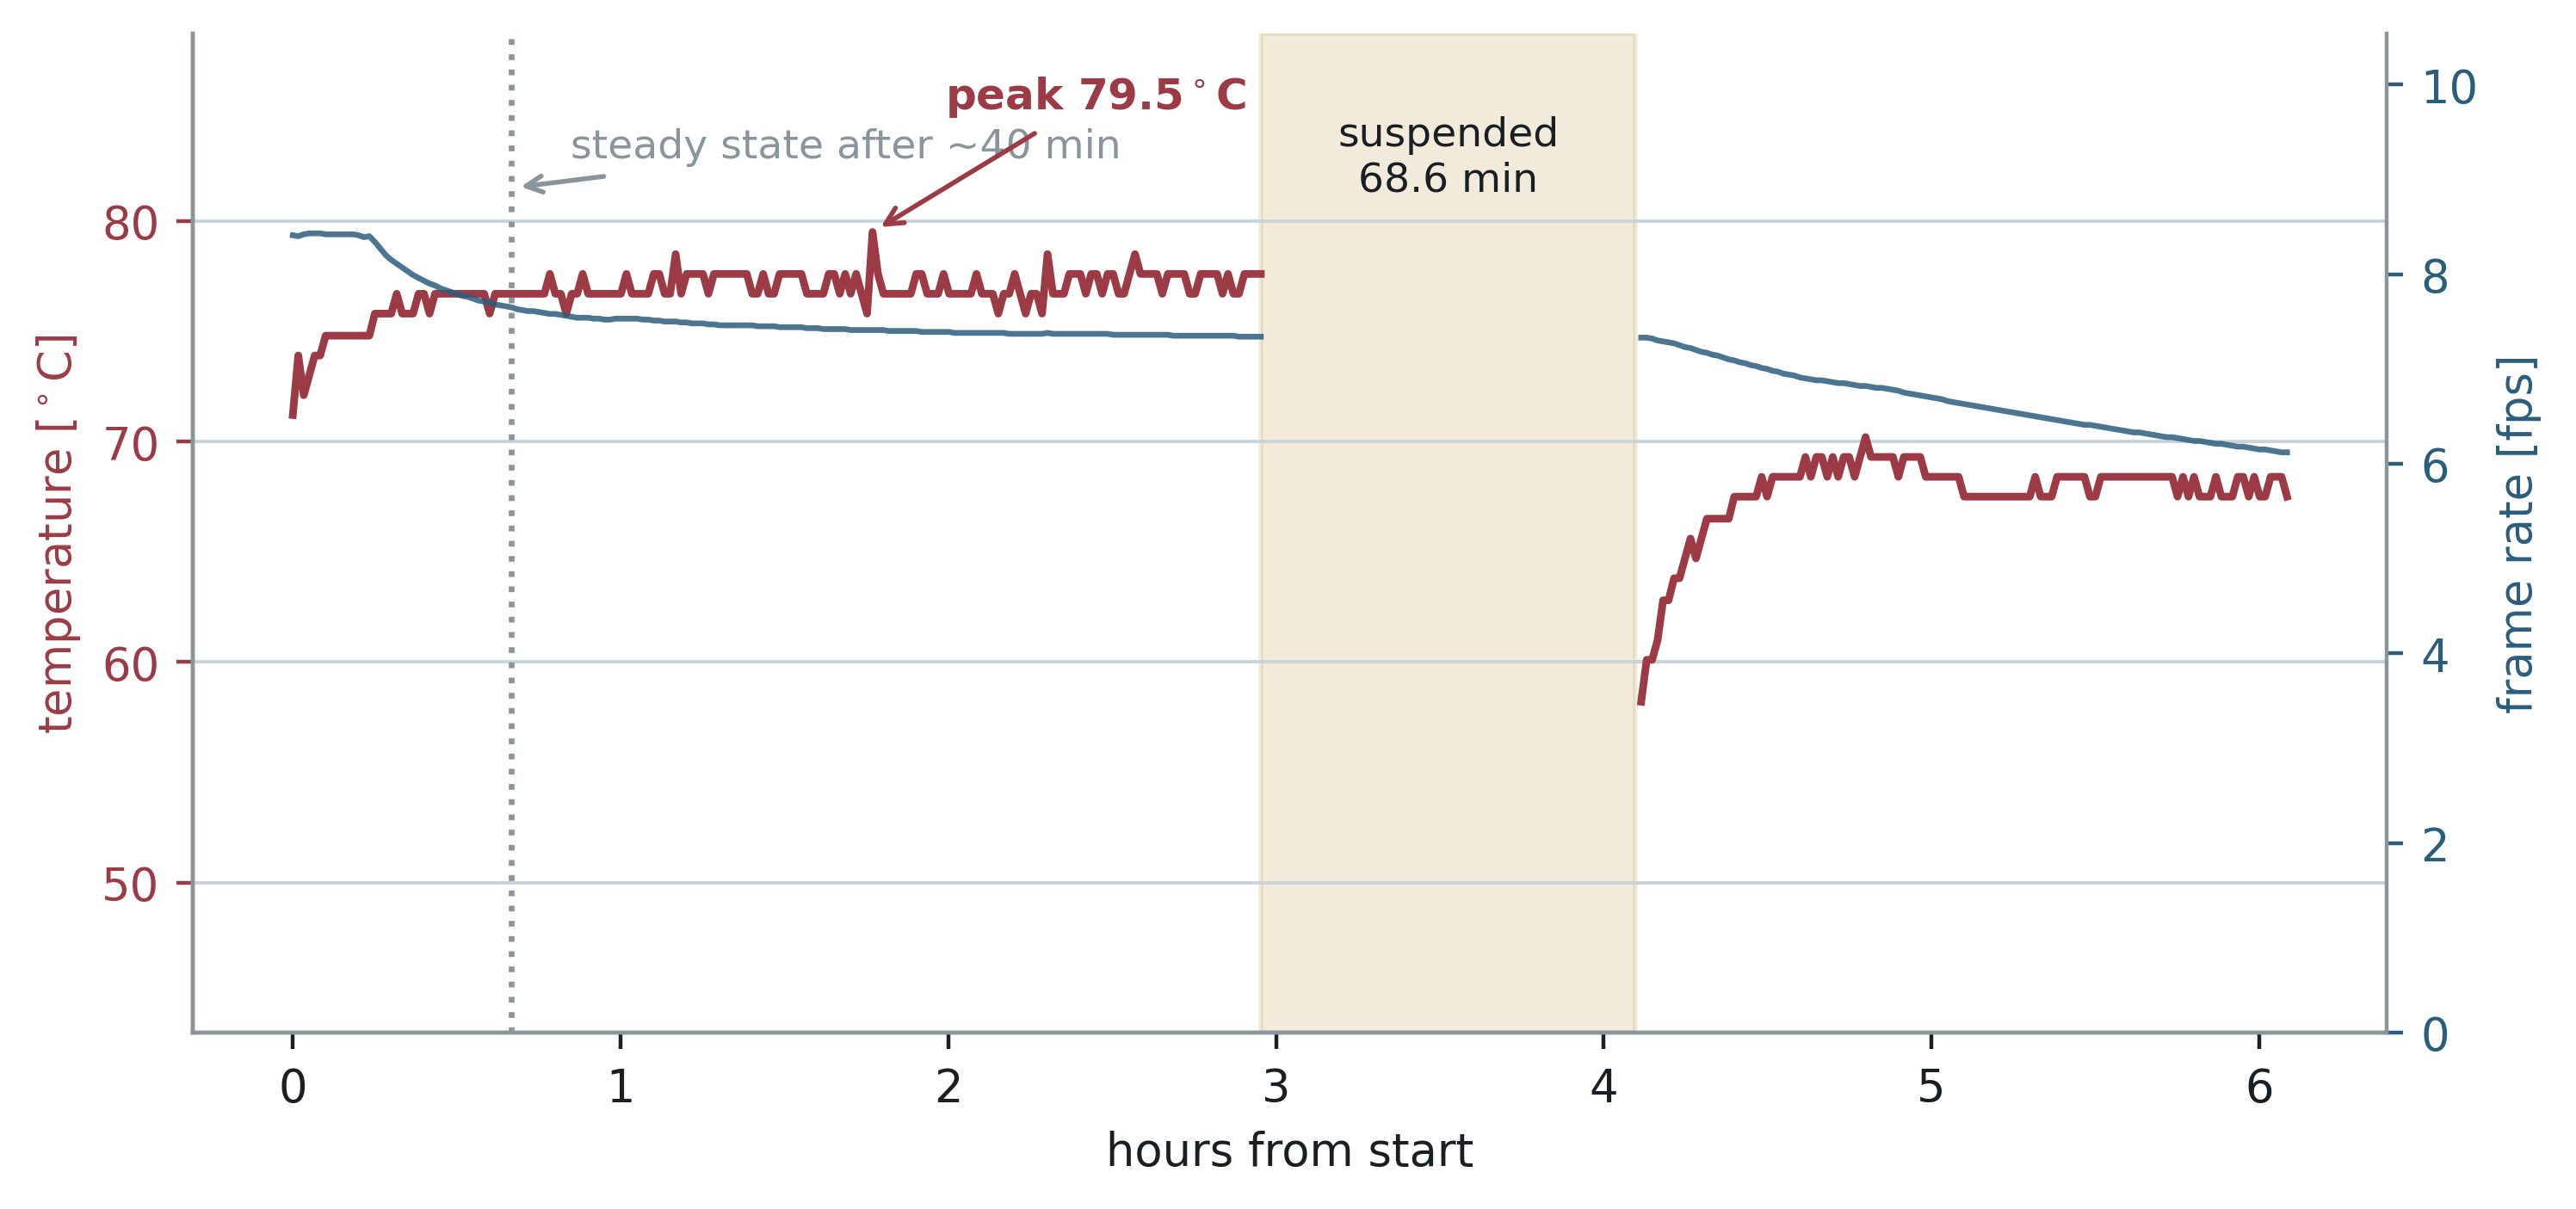
\includegraphics[width=0.85\textwidth]{figure/fig_termica_en.png}
\caption{Temperature of the device and processing cadence during the
prolonged domestic session of 11~August.}
\label{fig:termica}
\end{figure}

During this session, however, the operating system suspended for about 68 minutes. The program did not terminate and resumed execution after the wake-up. In order to make this problem observable, a check based on the comparison between system time and monotonic time was added.

It was moreover observed that the USB camera can be renumbered by the operating system, for example from \texttt{/dev/video0} to \texttt{/dev/video1}. In this case the program may remain active without receiving new frames. Capture is therefore monitored separately and, if no new frame arrives for more than 20~s, the camera is reopened.

A later trial, carried out on 6 September, covered 4,59~continuous hours. No suspensions of the operating system were detected. The camera dropped out twice, for about five seconds in total, and was reopened automatically. The mean cadence was 7,26~fps.

During this trial the system produced 14 events. They are not, however, counted as false alarms, because in that version of the recorder the frames around the alerts were not yet being retained, and it is therefore not possible to verify what actually happened. The 4,59-hour trial does not cover a whole night and therefore cannot demonstrate twelve hours of continuous operation.

\subsection{Resource budget}
\label{sec:risorse}

In Chapter~\ref{cap:contesto} computational and economic sustainability was listed among the requirements of the system. Table~\ref{tab:risorse} summarises the main resources demanded by the platform used.

\begin{table}[htbp]
\centering
\caption{Resource budget of the installed system.}
\label{tab:risorse}
\begin{tabular}{@{}p{4.6cm}p{9.0cm}@{}}
\toprule
\textbf{Quantity} & \textbf{Value} \\
\midrule
Platform & Radxa ROCK 4D, Rockchip RK3576 SoC \\
Memory available & 5.923~MB (6~GB nominal) \\
Accelerator & integrated NPU, 6~TOPS \\
Cost & of the order of 100~\euro{} per room, USB camera included \\
Model size & 606.409~bytes for the classifier, 1.175~bytes for the scaler; 607.584~bytes for everything needed to run \\
Cost per frame & Section~\ref{sec:costo-computazionale} \\
CPU / NPU split & Section~\ref{sec:stimatore} \\
Continuity of operation & Section~\ref{sec:continuita} \\
Memory used by the process & \textbf{297~MB} peak, that is 5\% of the memory available \\
\midrule
\textbf{Power consumption} & \textbf{not measured} \\
\bottomrule
\end{tabular}
\end{table}

The peak memory of the complete process is 297~MB, about 5\% of the memory available. Memory is therefore not a limitation for running the pipeline. The classifier is small as well, about 0,6~MB. The main computational cost therefore remains tied above all to pose estimation.

Power consumption was not measured. This quantity would require a direct measurement of the current drawn during operation and cannot be derived reliably from the specifications of the board alone.

A further limitation concerns $h_{\text{pav}}$. The floor reference is estimated using the frames in which the person is standing, and is therefore not available immediately after start-up. The effect was verified over 422 domestic sequences.

\begin{table}[H]
\centering
\caption{Availability of the classification with and without $h_{\text{pav}}$.}
\label{tab:pavimento_disponibilita}
\begin{tabular}{lcc}
\toprule
{} & \textbf{Sequences evaluated} & \textbf{Share} \\
\midrule
With $h_{\text{pav}}$ & 36 out of 422 & 8,5\% \\
Without $h_{\text{pav}}$ & 422 out of 422 & 100\% \\
\bottomrule
\end{tabular}
\end{table}

With $h_{\text{pav}}$ active, 91,5\% of the sequences produce no decision because the reference is not yet available. In the offline analyses of the domestic sequences the twelve-feature configuration, without $h_{\text{pav}}$, is therefore used. In continuous operation the problem concerns above all the initial phase, because the estimate is built only once. An alternative solution would be to calibrate the plane of the floor during installation.

\section{Validation in a domestic environment}
\label{sec:campo}

After the trials on the board, the system was left running in a domestic environment. The aim is to verify the behaviour of the pipeline during longer acquisitions and with activities different from those in the dataset, in which the environment, the lighting, the position of the people and above all the frequency of falls change, the latter being far lower during real use than in an experimental dataset.

\subsection{Protocol of the domestic sessions}
\label{sec:protocollo-campo}

Before the domestic trials, the configuration in use produced 46 false positives over 4.767 negative windows, that is 0,96\%. In the dataset this value can be compatible with good precision, because the share of positive examples is far greater than it would be during ordinary domestic use. When the system is left running for many hours, by contrast, even a low error rate is applied to a very large number of windows.
At 9~fps, with a window of 22 samples and a stride of two, a new decision is produced every $2/9 \simeq 0,22$~s, for a total of about 388.800 windows per day.

\begin{table}[ht]
\centering
\caption{Projection of the false positive rate over one day of continuous operation, as observed on the dataset.}
\label{tab:falsi_positivi_giorno}
\begin{tabular}{lrr}
\toprule
\textbf{Windowing} & \textbf{Windows/day} &
\textbf{False positives/day} \\
\midrule
Non-overlapping & $\sim35{.}345$ & $\sim341$ \\
With a stride of 2 samples & $\sim388{.}800$ & $\sim3{.}751$ \\
\bottomrule
\end{tabular}
\end{table}

The two cases correspond to about 14 and 156 positive windows per hour. These are not, however, distinct alarms, because several consecutive windows may belong to the same episode. The calculation therefore serves to show why the false positive rate per window is not enough to evaluate a continuous system. Twelve blocks were recorded, spread over four days and two private homes, for a total duration of 9,6~hours.

\begin{table}[htbp]
\centering
\caption{Protocol of the domestic sessions.}
\label{tab:protocollo_domestico}
\begin{tabular}{@{}p{5.0cm}p{8.6cm}@{}}
\toprule
\textbf{Item} & \textbf{Value} \\
\midrule
Environments & 2 private homes \\
Days & 4 \\
Blocks recorded & 12 \\
Total duration & about 9,6 hours \\
Position of the camera & lateral with respect to the area of movement, optical axis roughly horizontal, 1,2--1,5~m above the floor \\
Activities & ordinary daily activities, sitting down quickly, bending over, lying down voluntarily and the presence of several people \\
Falls & 5 across the 12 sessions, all simulated \\
Ground truth & temporal annotation of the falls alone \\
Participants & total number not recorded; there are blocks with one, two and three people in view at the same time \\
Size of the environments & not recorded \\
Hours with a valid pose & 7,45 out of 9,58 ($77,8\%$) \\
\bottomrule
\end{tabular}
\end{table}

The twelve blocks described here constitute the August acquisition campaign, and their total duration is reported as effective operating time. The analysis of alarm events in Section~\ref{sec:finestre-eventi} uses a partly different set, and the two should not be confused. That analysis considers nine sessions: the eight August blocks longer than nine minutes, which alone are long enough for a rate per hour to be meaningful, together with the prolonged board session of 6 September, recorded later and therefore absent from this campaign. It also counts wall-clock time rather than effective operating time. The two accounting bases differ mainly for the session of 11 August, which lasted 6,11~hours of wall clock but only 4,99~hours of effective operation, the difference being the 68-minute suspension of the operating system described in Section~\ref{sec:continuita}.

The acquisitions comprise ordinary daily activities, five simulated falls and some activities chosen deliberately because they are potentially ambiguous, such as sitting down quickly, bending over and lying down voluntarily, and the simultaneous presence of several people. The camera was placed laterally with respect to the main area of movement, about 1,2--1,5~m above the floor. The distance was chosen so as to keep the person visible both when standing and when on the ground.

\begin{figure}[htbp]
\centering
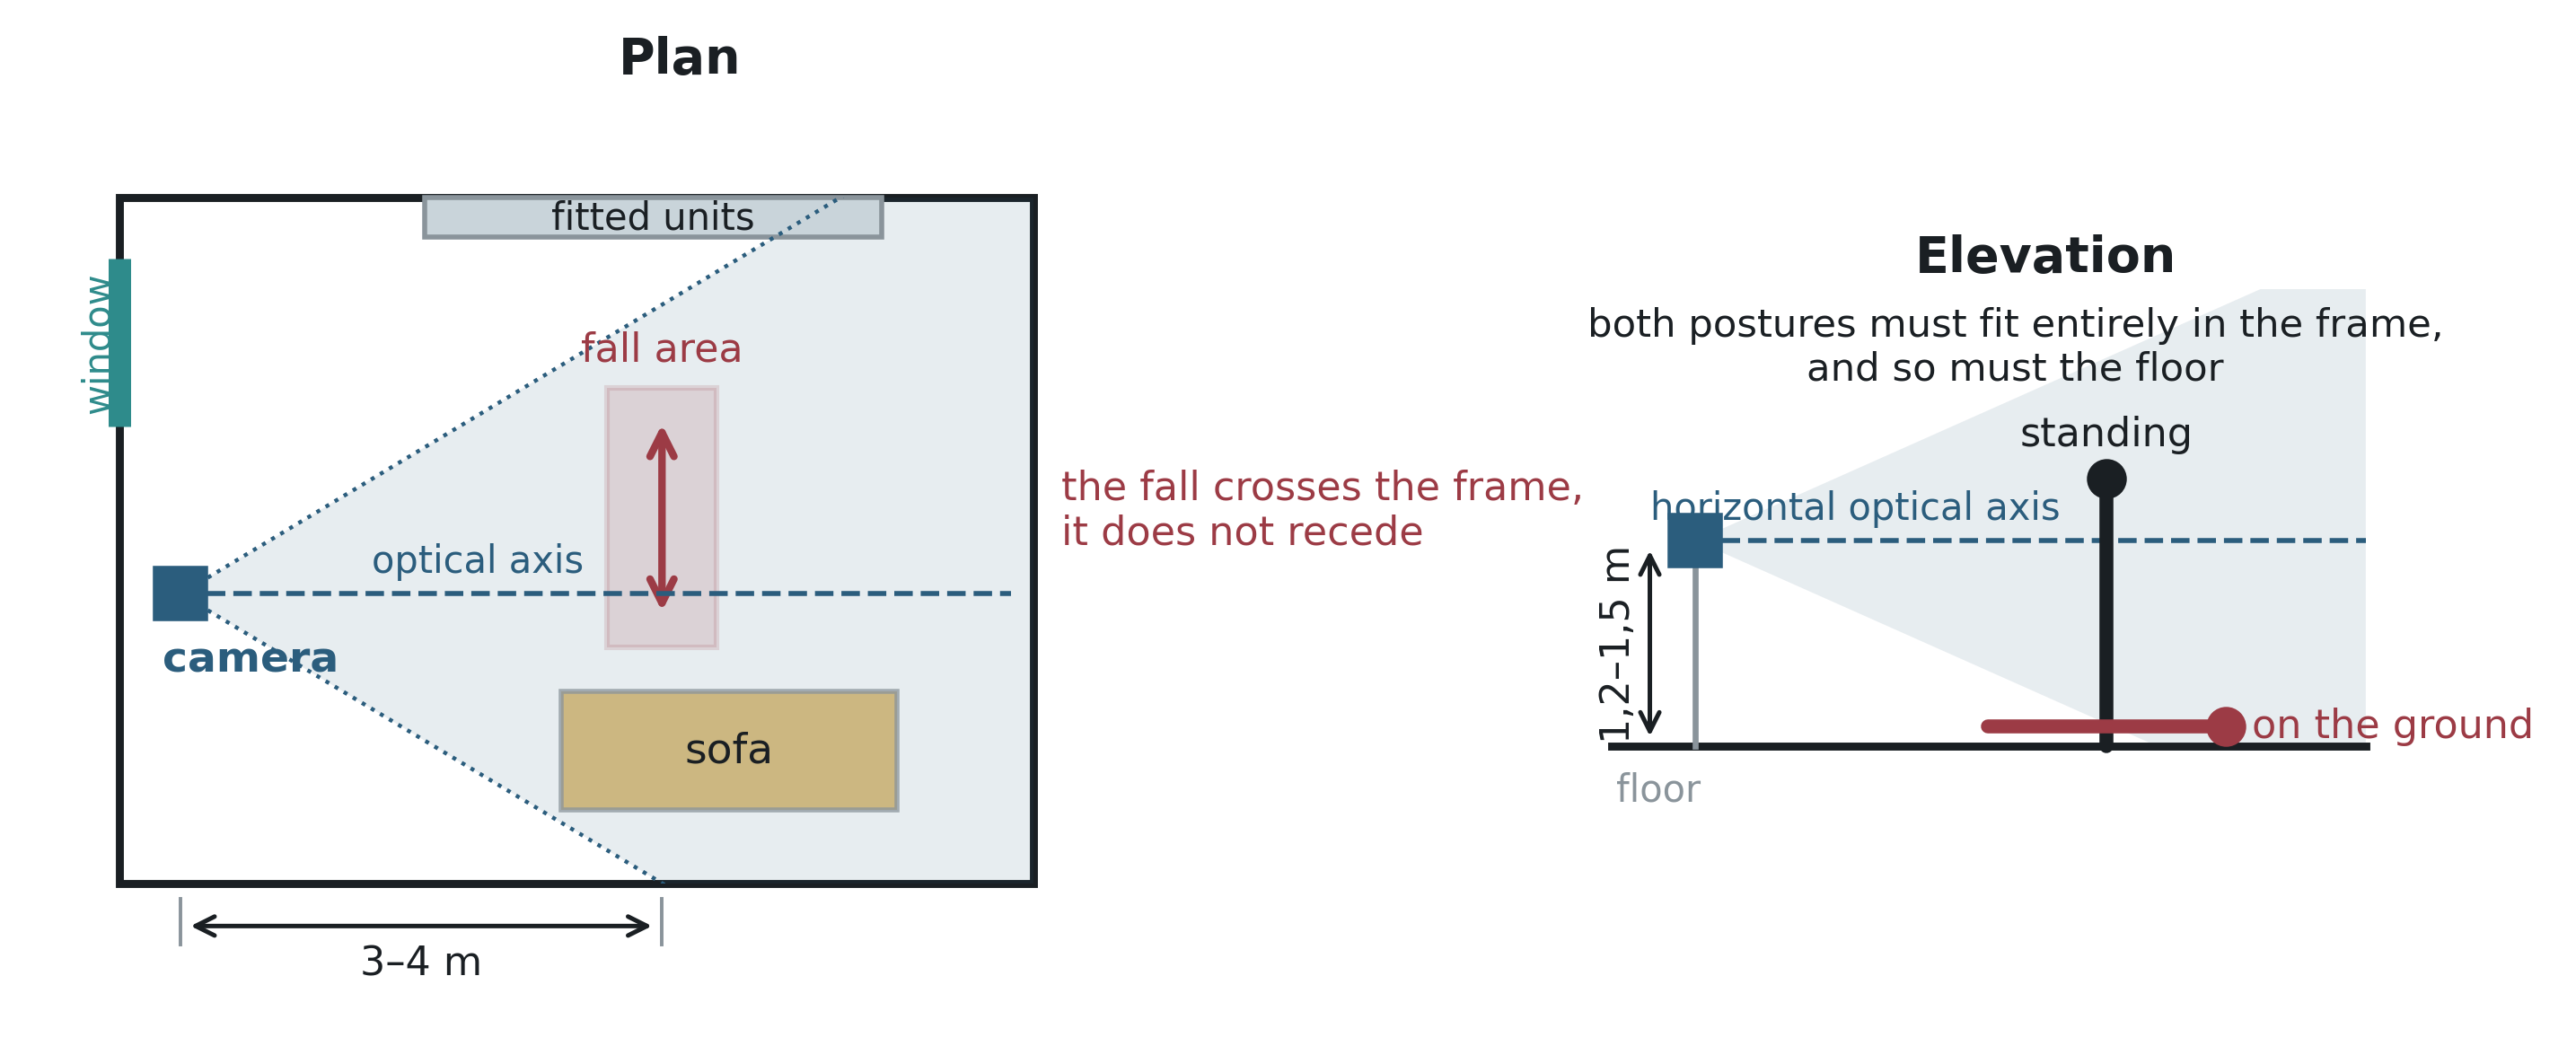
\includegraphics[width=0.85\textwidth]{figure/fig_stanza_en.png}
\caption{Layout scheme used during the domestic acquisitions.}
\label{fig:stanza}
\end{figure}

The system saves pose, features and classifier scores. The RGB images are retained locally only in the vicinity of the alerts, so that errors can be checked afterwards. The complete video stream is therefore neither transmitted nor stored continuously.

The acquisitions were carried out in real homes, with the lighting and the furnishings present in those environments and during ordinary daily activities.
The five falls considered in the first evaluation are all simulated. The elderly participants were not asked to perform falls; their recordings contain only ordinary daily activities, including situations in which the person remains lying on a sofa. These acquisitions therefore reproduce realistic domestic conditions, but do not constitute a clinical validation on natural falls.

\subsection{Quality of the acquisitions and usable data}

The continuous presence of people in the frame was not annotated. It is therefore not possible to measure directly the actual hours of people in the scene. What can be computed is the time during which the estimator returned a valid pose: 7,45~hours out of the 9,58 recorded, that is 77,8\%. This is a lower bound on the time of presence, because a person may be in the frame without producing a valid pose, for example when part of the body leaves the image.

\begin{table}[ht]
\centering
\caption{Share of frames with a valid pose across the days of acquisition.}
\label{tab:qualita_pose_domestiche}
\begin{tabular}{lll}
\toprule
\textbf{Day} & \textbf{Place} & \textbf{Valid poses} \\
\midrule
10 August & first home & 0,6--39,8\% \\
11 August & first home & 83,0\% \\
12 August & second home & 86,8--99,3\% \\
13 August & second home & 25,9--97,6\% \\
\bottomrule
\end{tabular}
\end{table}

The six blocks recorded on 10 August have a percentage of valid poses between 0,6\% and 39,8\%. The camera was too close and parts of the body often left the frame. These blocks are not used in the quantitative results that follow. On the following days the framing was widened.

\section{Event-level metrics}
\label{sec:falsi-allarmi}
\label{sec:finestre-eventi}

The classifier produces a probability for every temporal window. In continuous operation, however, several consecutive windows may exceed the threshold during the same fall or during the same activity. Treating every positive window as a new alarm would therefore overestimate the number of alerts received by the user. For this reason the decisions on the windows are kept distinct from the alarm events.

\subsection{From windows to alarm events}

The classifier produces a probability for every temporal window, but several consecutive windows may refer to the same activity. For this reason
we do not treat every window above the threshold as a new alarm, but
generate an alarm when at least five consecutive windows exceed the decision threshold.

After the alarm, a suspension interval of 30~s is applied, during which any subsequent positive windows are treated as part of the same episode.

The set used from here on comprises nine sessions, counted in wall-clock time: the eight blocks of the August campaign of Table~\ref{tab:protocollo_domestico} that exceed nine minutes, and the prolonged board session of 6 September. The four shortest August blocks, lasting between two and seven minutes, are excluded because a rate per hour computed on them would not be meaningful. The recordings were not all acquired with the same threshold: four of the nine sessions used $0{,}45$ and five used $0{,}50$.

Recomputing all the sessions with a threshold of $0{,}50$, the overall ratio between windows above the threshold and events changes by about 1\%. The difference therefore does not alter the conclusions, but it is kept explicit. Over the nine sessions used for this analysis, for a total duration of 14,98~hours, the ratio between windows above the threshold and events is 44,8.

\begin{figure}[htbp]
\centering
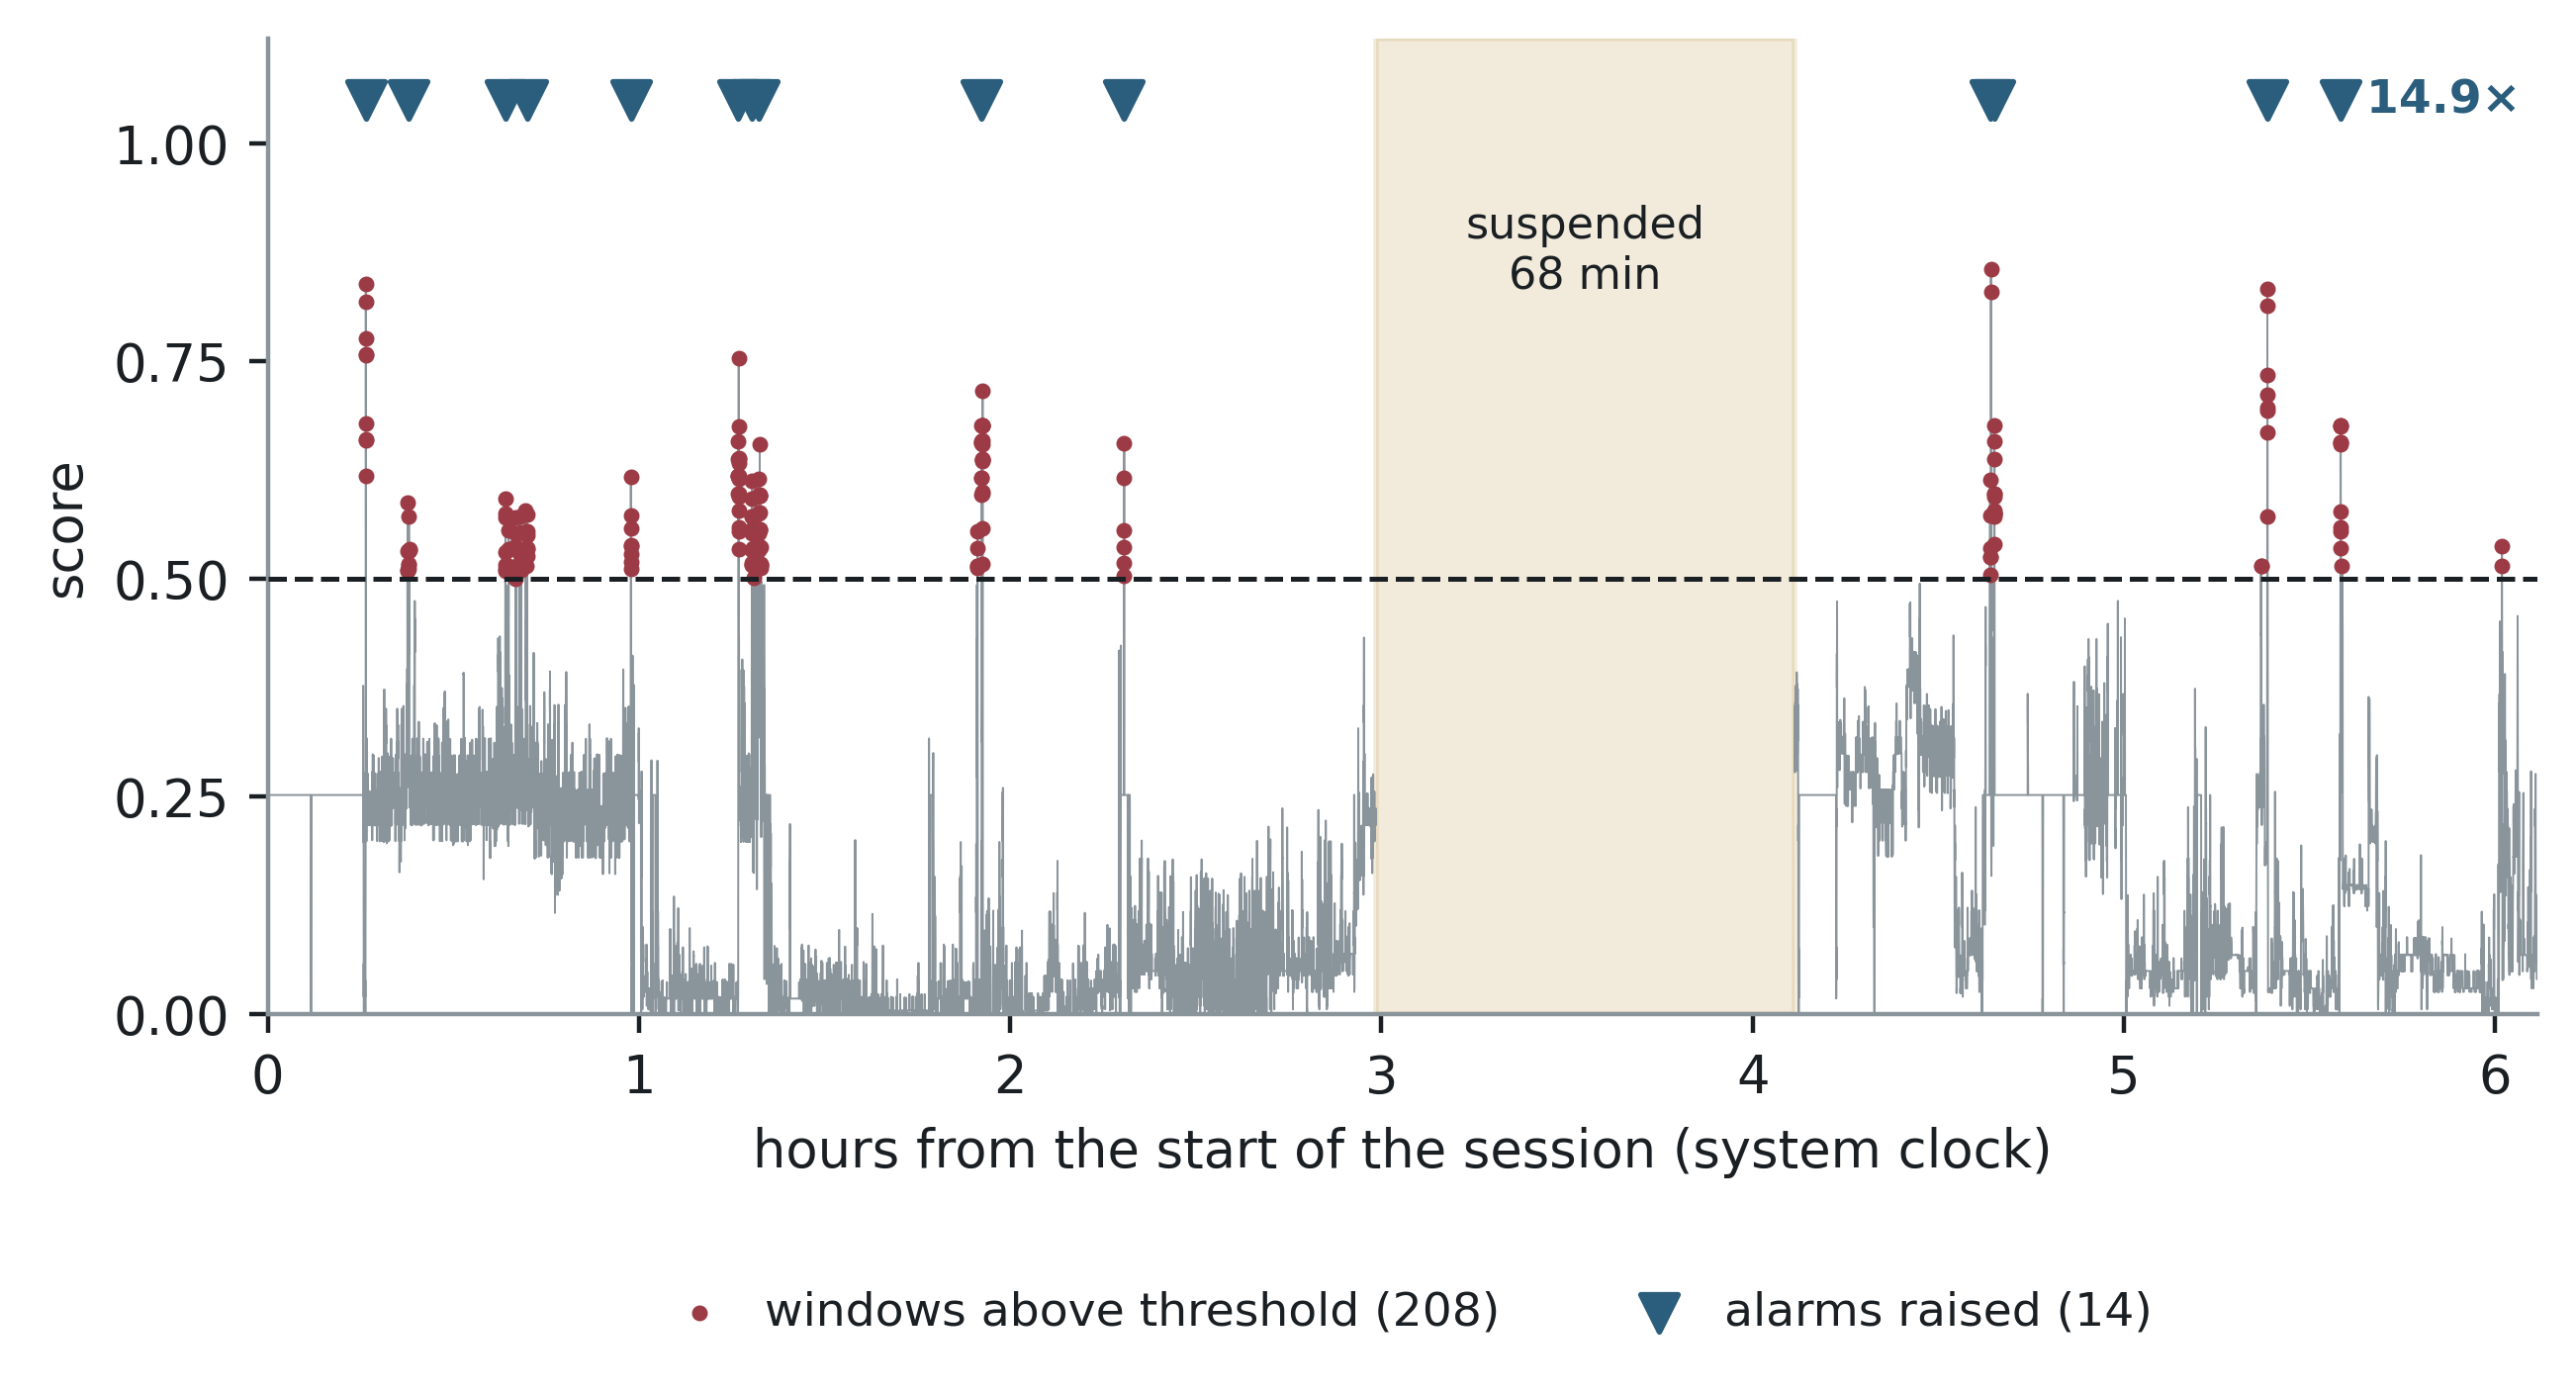
\includegraphics[width=0.85\textwidth]{figure/fig_sessione_en.png}
\caption{Positive windows and events generated during a prolonged session.}
\label{fig:sessione}
\end{figure}

In the session of 11 August shown in Figure~\ref{fig:sessione}, 208 windows above the threshold and 14 events generated are observed, a ratio of 14,9. The value differs from the overall ratio of 44,8 because the duration of the positive sequences changes from one recording to another. For the domestic trials the number of events per hour was therefore used as the main operational measure, keeping the number of windows above the threshold separate.

The latter remains useful for distinguishing a brief error from a persistent state. A person lying on a sofa, for example, may keep the score high for a prolonged period. The suspension interval reduces the number of alerts, but the classifier may go on interpreting that configuration as positive.

\subsection{Recall and criteria for associating the events}
\label{sec:recall-campo}

The five simulated falls were annotated only to the minute. In order to associate them with the alarms, the temporal tolerance and the persistence required were therefore varied.

\begin{table}[ht]
\centering
\caption{Falls associated with a detection as the criterion used varies.}
\label{tab:associazione_cadute}
\begin{tabular}{lcc}
\toprule
\textbf{Tolerance} &
\textbf{Persistence 1} &
\textbf{Persistence 5} \\
\midrule
$\pm10$ s & 0/5 & 0/5 \\
$\pm30$ s & 2/5 & 2/5 \\
$\pm60$ s & 4/5 & 2/5 \\
$\pm90$ s & 4/5 & 2/5 \\
\bottomrule
\end{tabular}
\end{table}

The result of 4/5 is obtained with a tolerance of $\pm60$~s and by treating a single positive window as sufficient. The first positive windows of the four falls recognised appear at $11{,}8$, $19{,}4$, $27{,}7$ and $32{,}3$~s from the annotated minute. The resulting recall is $0{,}80$, with a 95\% confidence interval running from $0{,}28$ to $0{,}99$. With only five falls the value is therefore very uncertain.

With the operational rule of five consecutive windows, by contrast, two of the five falls generate an event. The other three produce runs of two, three and zero positive windows, below the persistence threshold. Recall must therefore always be reported together with the association criterion used.

A difference was moreover found during this check between the offline analysis and the one carried out on the board. The first analysis indicated two falls recognised out of five, whereas during execution on the device four were obtained. The difference depended on two aspects. In the offline analysis the mean of the models obtained during cross-validation was used, whereas the model installed on the board was the final one, retrained on the whole set available. In addition, the subsampling from 18 to 9~fps was applied a second time to the board recordings. Once these two differences had been removed, the offline analysis reproduces the behaviour observed on the device.

A more precise check was possible in the session of 9 September, in which four simulated falls were annotated directly on the frames. The classifier recognises three of the four falls, while the aggregation rule generates two alarm events. Figures~\ref{fig:sessione_v5_andamento} and~\ref{fig:sessione_v5_cadute} show respectively the course of the whole session and the detail of the falls.

\begin{figure}[htbp]
\centering
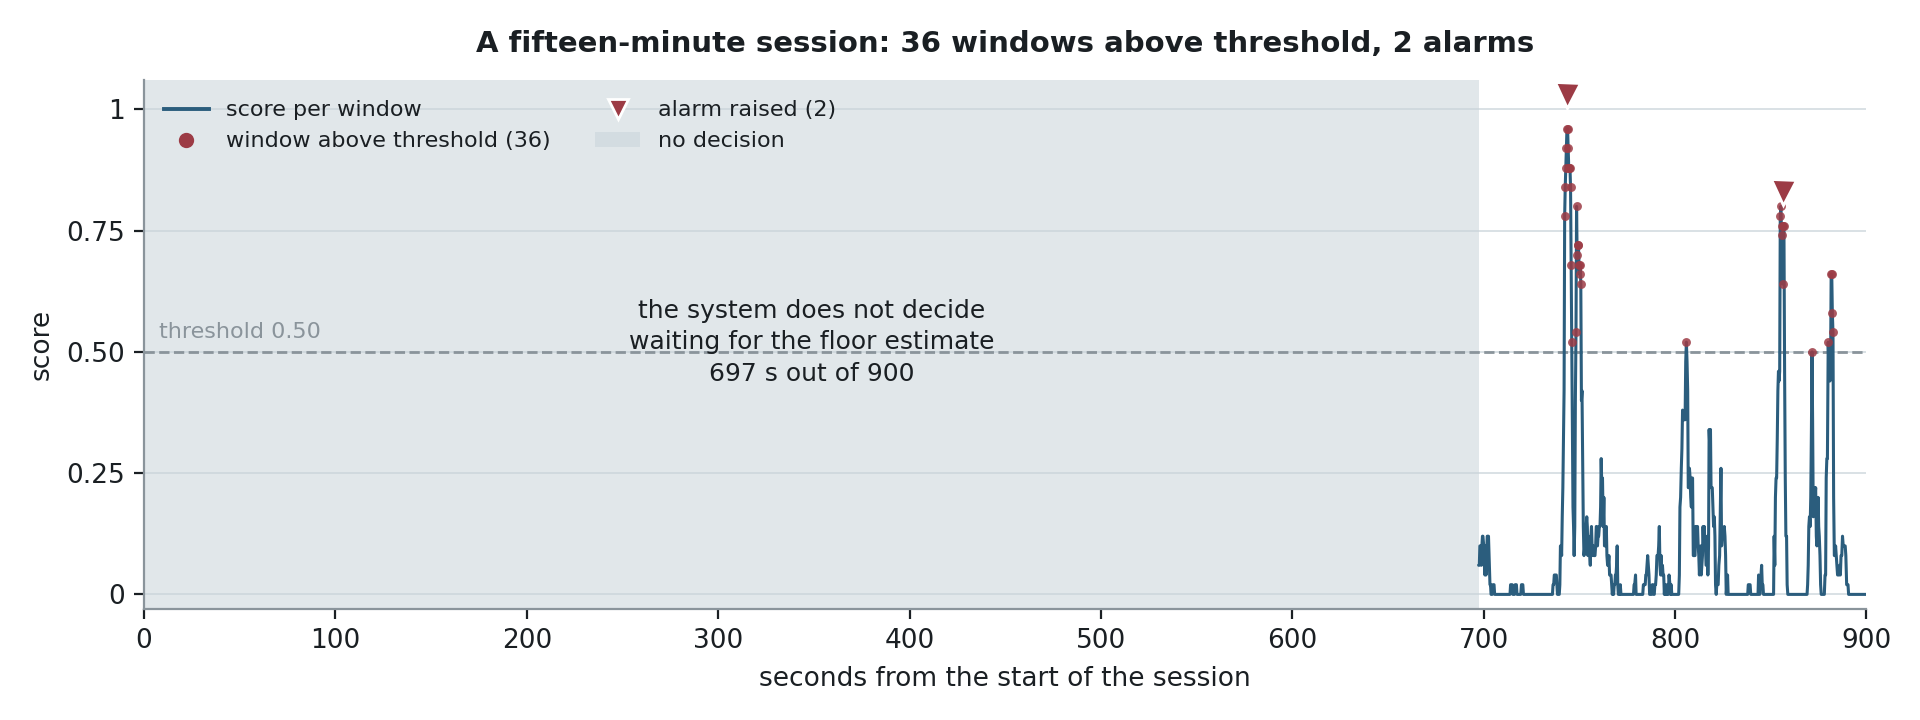
\includegraphics[width=.96\textwidth]{figure/fig_sessione_v5_andamento_en.png}
\caption{Course of the score during the session of 9 September. In the first 697~s the system produces no decisions, because the plane of the floor is not yet available. In the 203~s that follow, 624 windows are produced, 36 of them above the threshold, and two alarm events}
\label{fig:sessione_v5_andamento}
\end{figure}

\begin{figure}[htbp]
\centering
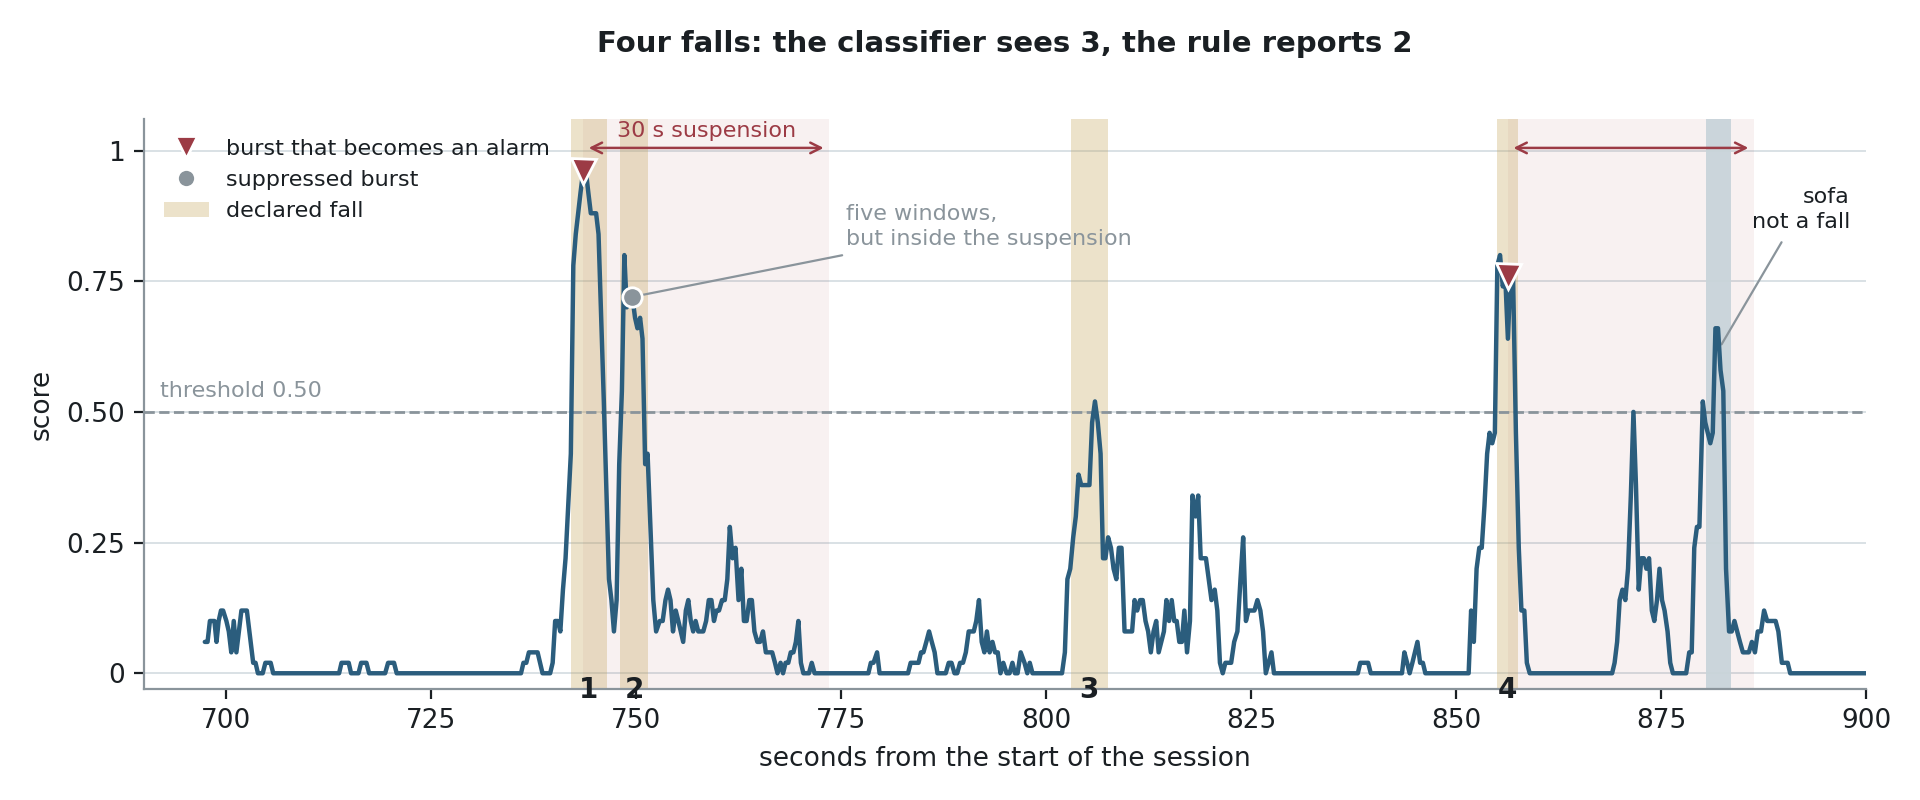
\includegraphics[width=.96\textwidth]{figure/fig_sessione_v5_cadute_en.png}
\caption{Detail of the four simulated falls and of the false positive associated with the sofa in the session of 9 September}
\label{fig:sessione_v5_cadute}
\end{figure}

The first fall produces a sufficient run of windows above the threshold and correctly generates an alarm. Figure~\ref{fig:caduta_board} shows a frame from the same sequence, with the skeleton and the score produced directly by the board.

\begin{figure}[htbp]
\centering
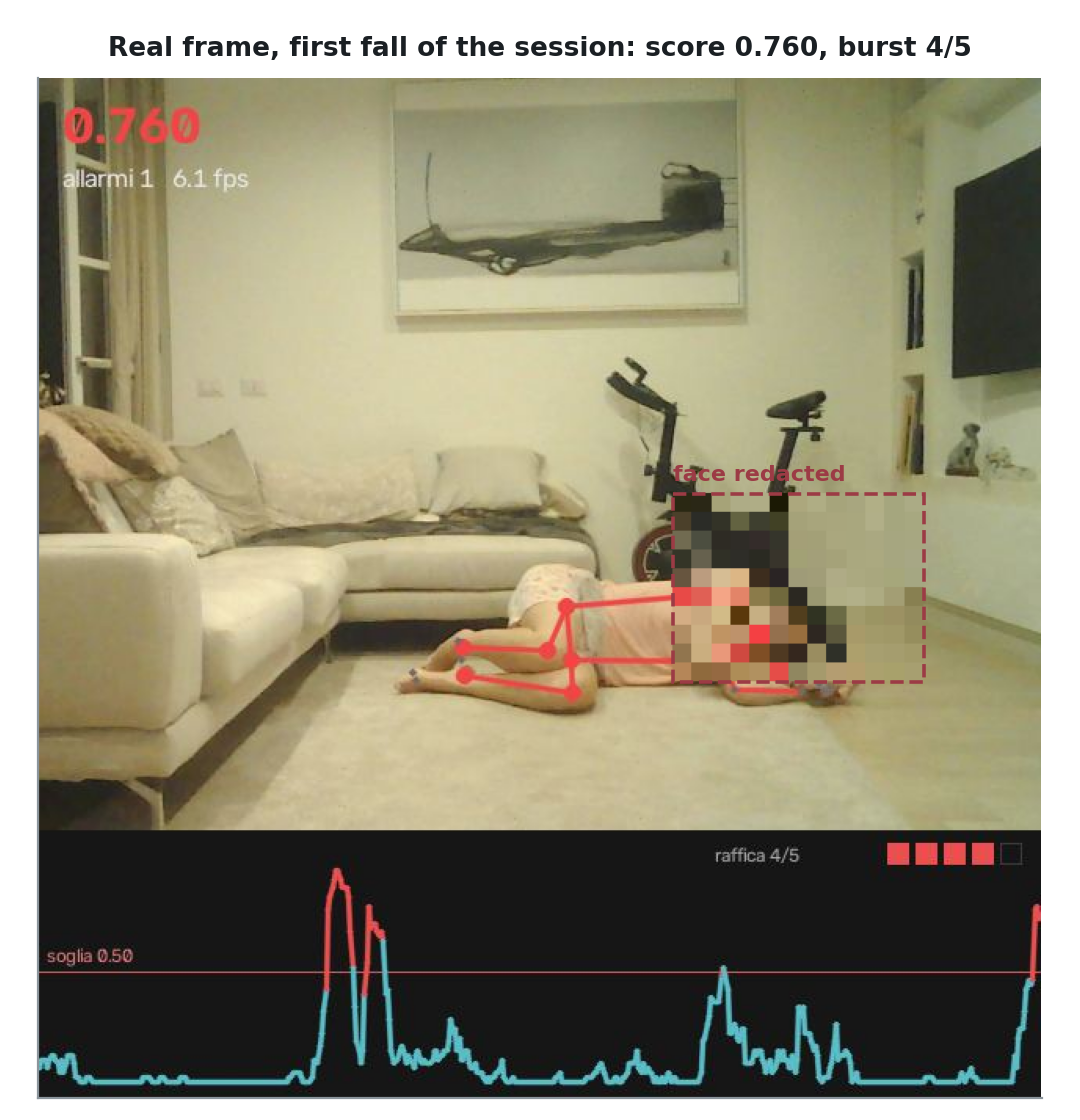
\includegraphics[width=0.75\textwidth]{figure/fig_caduta_board_en.png}
\caption{Real frame from the session of 9 September, with the skeleton and the score produced by the board. The overlay is the one the device draws in real time.}
\label{fig:caduta_board}
\end{figure}

The second fall occurs about six seconds after the first. The classifier recognises it, but no new alarm is generated because the system is still within the 30~s suspension interval. This case shows an important difference between an error of the classifier and an error of the aggregation logic: the fall was recognised by the model, but suppressed by the operational rule.

In the same session a person sitting on the sofa produces a run of four windows above the threshold. No alarm is generated, because the five consecutive windows required are not reached. Persistence therefore removes some false positives, but it can also suppress real events that are very close in time.

\subsection{Detection latency}
\label{sec:latenza}

Another important quantity is the latency, which ought to be measured between the beginning of the fall and the generation of the alarm. In the first domestic recordings this value cannot be obtained directly, because the falls are annotated only to the minute.

In the four falls recognised, the first positive window appears at 11,8, 19,4, 27,7 and 32,3~s respectively with respect to the annotated minute. These values do not, however, represent the latency of the system, because the exact second at which the fall began is not known.

What can be computed instead is the time introduced by the configuration of the pipeline. Considering a mean frequency of 8,02~fps, a window of 22 samples and a persistence of five consecutive windows, the following decomposition is obtained.

\begin{table}[ht]
\centering
\caption{Decomposition of the time introduced by the configuration of the pipeline at the mean frequency of 8,02~fps.}
\label{tab:latenza}
\begin{tabular}{lrr}
\toprule
\textbf{Component} & \textbf{Time} & \textbf{Share} \\
\midrule
Computation per frame & 0,125 s & 3,2\% \\
Filling of the window & 2,743 s & 71,0\% \\
Persistence & 0,997 s & 25,8\% \\
\midrule
Total & 3,865 s & 100\% \\
\bottomrule
\end{tabular}
\end{table}

The largest contribution is due to the filling of the window, 2,743~s. The computation per frame accounts for only 3,2\% of the total. Latency therefore depends above all on the length of the window and on the persistence required in order to generate the alarm. Reducing the processing time alone would have a smaller effect than changing these two parameters.

The value of 0,997~s represents the minimum time needed to obtain five consecutive windows. In the two falls for which the whole sequence is available, the time observed is instead 1,70 and 1,28~s. Some windows drop temporarily below the threshold, restarting the count.
With the annotations available it is therefore possible to estimate the time introduced by the pipeline, but not the full latency between the physical beginning of the fall and the alert.

\section{Comparison between benchmark and real behaviour}
\label{sec:rovesciamento}
\label{sec:confronto-domini}

Finally, the same configurations were compared on the benchmark and in the domestic recordings. The metrics used in the two cases are different, so the absolute values are not compared directly: what we observe is how the difference between the configurations changes in going from the dataset to the domestic environment.

\subsection{Comparison of the configurations}

Five configurations built on representation A3 were considered. A3h adds the height above the floor, A3i introduces the integral quantities, while the configurations with counter-examples also use negative examples collected in the domestic recordings.

The feature $h_{\text{pav}}$ had not been selected initially. It was reintroduced after false positives had been observed on people lying on raised surfaces. The result obtained on the same recordings is therefore not regarded as a verification independent of that choice.

\begin{table}[ht]
\centering
\caption{Comparison of the configurations on the benchmark and in the domestic recordings.}
\label{tab:configurazioni}
\begin{tabular}{lccc}
\toprule
\textbf{Configuration} &
\textbf{$F_2$ laboratory} &
\textbf{Windows/hour at home} &
\textbf{Falls} \\
\midrule
A3 & $0{,}898\pm0{,}075$ & 139,9 & 3/5 \\
A3h & $0{,}931\pm0{,}051$ & 70,4 & 2/5 \\
A3h + counter-examples & $0{,}942\pm0{,}060$ & 2,1 & 2/5 \\
A3i & $0{,}943\pm0{,}064$ & 9,8 & 4/5 \\
A3i + counter-examples & $0{,}953\pm0{,}055$ & 2,7 & 3/5 \\
\bottomrule
\end{tabular}
\end{table}

On the benchmark every configuration improves on A3. Between A3 and A3i with counter-examples the difference in $F_2$ is 0,055, of the same order as the variability between subjects. In the domestic recordings, by contrast, the positive windows went from 139,9 to 2,7 per hour, about 52 times fewer. The individual types of error also improve on the benchmark.

\begin{table}[ht]
\centering
\caption{False negatives and false positives of the five configurations in the LOSO evaluation on ten subjects.}
\label{tab:errori_configurazioni}
\begin{tabular}{lcccc}
\toprule
\textbf{Configuration} & \textbf{$F_2$} &
\textbf{Recall} & \textbf{FN} & \textbf{FP} \\
\midrule
A3 & 0,898 & 0,929 & 45 & 172 \\
A3h & 0,931 & 0,962 & 22 & 137 \\
A3h + counter-examples & 0,942 & 0,965 & 22 & 129 \\
A3i & 0,943 & 0,977 & 14 & 150 \\
A3i + counter-examples & 0,953 & 0,980 & 14 & 124 \\
\bottomrule
\end{tabular}
\end{table}

Going from A3 to A3i with counter-examples, the false negatives fall from 45 to 14 and the false positives from 172 to 124. The improvement in recall is therefore not obtained by increasing the false positives.

\subsection{Analysis of the differences between the two domains}

The main difference between the dataset and the domestic recordings concerns the negative activities with people in a horizontal position. In the dataset these activities take place mostly close to the floor. In the domestic recordings a person may instead be lying on a bed or a sofa.

\begin{table}[htbp]
\centering
\caption{Qualitative distribution of the negative configurations with a person in a horizontal position.}
\label{tab:negativi_orizzontali}
\begin{tabular}{lcc}
\toprule
\textbf{Domain} & \textbf{Approximate share} &
\textbf{Prevailing position} \\
\midrule
Laboratory & about a fifth & floor \\
Domestic environment & about half & raised surface \\
\bottomrule
\end{tabular}
\end{table}

The median height of the hips in the horizontal negatives is about $+0{,}02$ trunk lengths in the dataset and $+1{,}47$ in the domestic recordings.
This difference explains why $h_{\text{pav}}$ has a limited effect on the benchmark but turns out more useful in the domestic recordings. A benchmark can only assess the conditions present in its own data. If a situation typical of the real environment is poorly represented, a feature designed to distinguish it may have a reduced effect during the evaluation on the dataset.

\subsection{Transfer of the counter-examples}

The domestic counter-examples were collected in the same two homes used for the evaluation. In order to check whether the improvement depended on the individual room alone, the model was trained with the counter-examples of one home and evaluated in the other.

\begin{table}[ht]
\centering
\caption{Transfer of the counter-examples between the two homes.}
\label{tab:trasferimento_controesempi}
\begin{tabular}{lcc}
\toprule
\textbf{Counter-examples used} &
\textbf{Test home} &
\textbf{Events/hour} \\
\midrule
None / home 2 & home 1 & $0{,}342 \rightarrow 0{,}171$ \\
None / home 1 & home 2 & $1{,}781 \rightarrow 0{,}890$ \\
\bottomrule
\end{tabular}
\end{table}

In both cases the number of events per hour roughly halves. The improvement therefore does not depend on the room in which the examples were collected alone. With only two homes it is not, however, possible to verify generalisation to new environments. The counter-examples must therefore be regarded as a form of adaptation to the domestic domain. Moreover, with A3i, adding the counter-examples brings the falls recognised from 4/5 to 3/5. The same trade-off was observed when the three definitions of the task were compared.

\begin{table}[ht]
\centering
\caption{Behaviour of the three definitions of the task in the domestic recordings.}
\label{tab:compiti_domestici}
\begin{tabular}{lcc}
\toprule
\textbf{Task} & \textbf{Alarm events/hour} &
\textbf{Falls detected} \\
\midrule
Event & 1,6 & 3/5 \\
State & 29,5 & 0/5 \\
Alarm & 36,4 & 4/5 \\
\bottomrule
\end{tabular}
\end{table}

The \emph{event} task produces 1,6 events per hour, against 29,5 for the \emph{state} task and 36,4 for the \emph{alarm} task, but it recognises one fall fewer than the alarm task. Here too it is therefore not possible to evaluate a configuration by considering a single metric.

\begin{figure}[htbp]
\centering
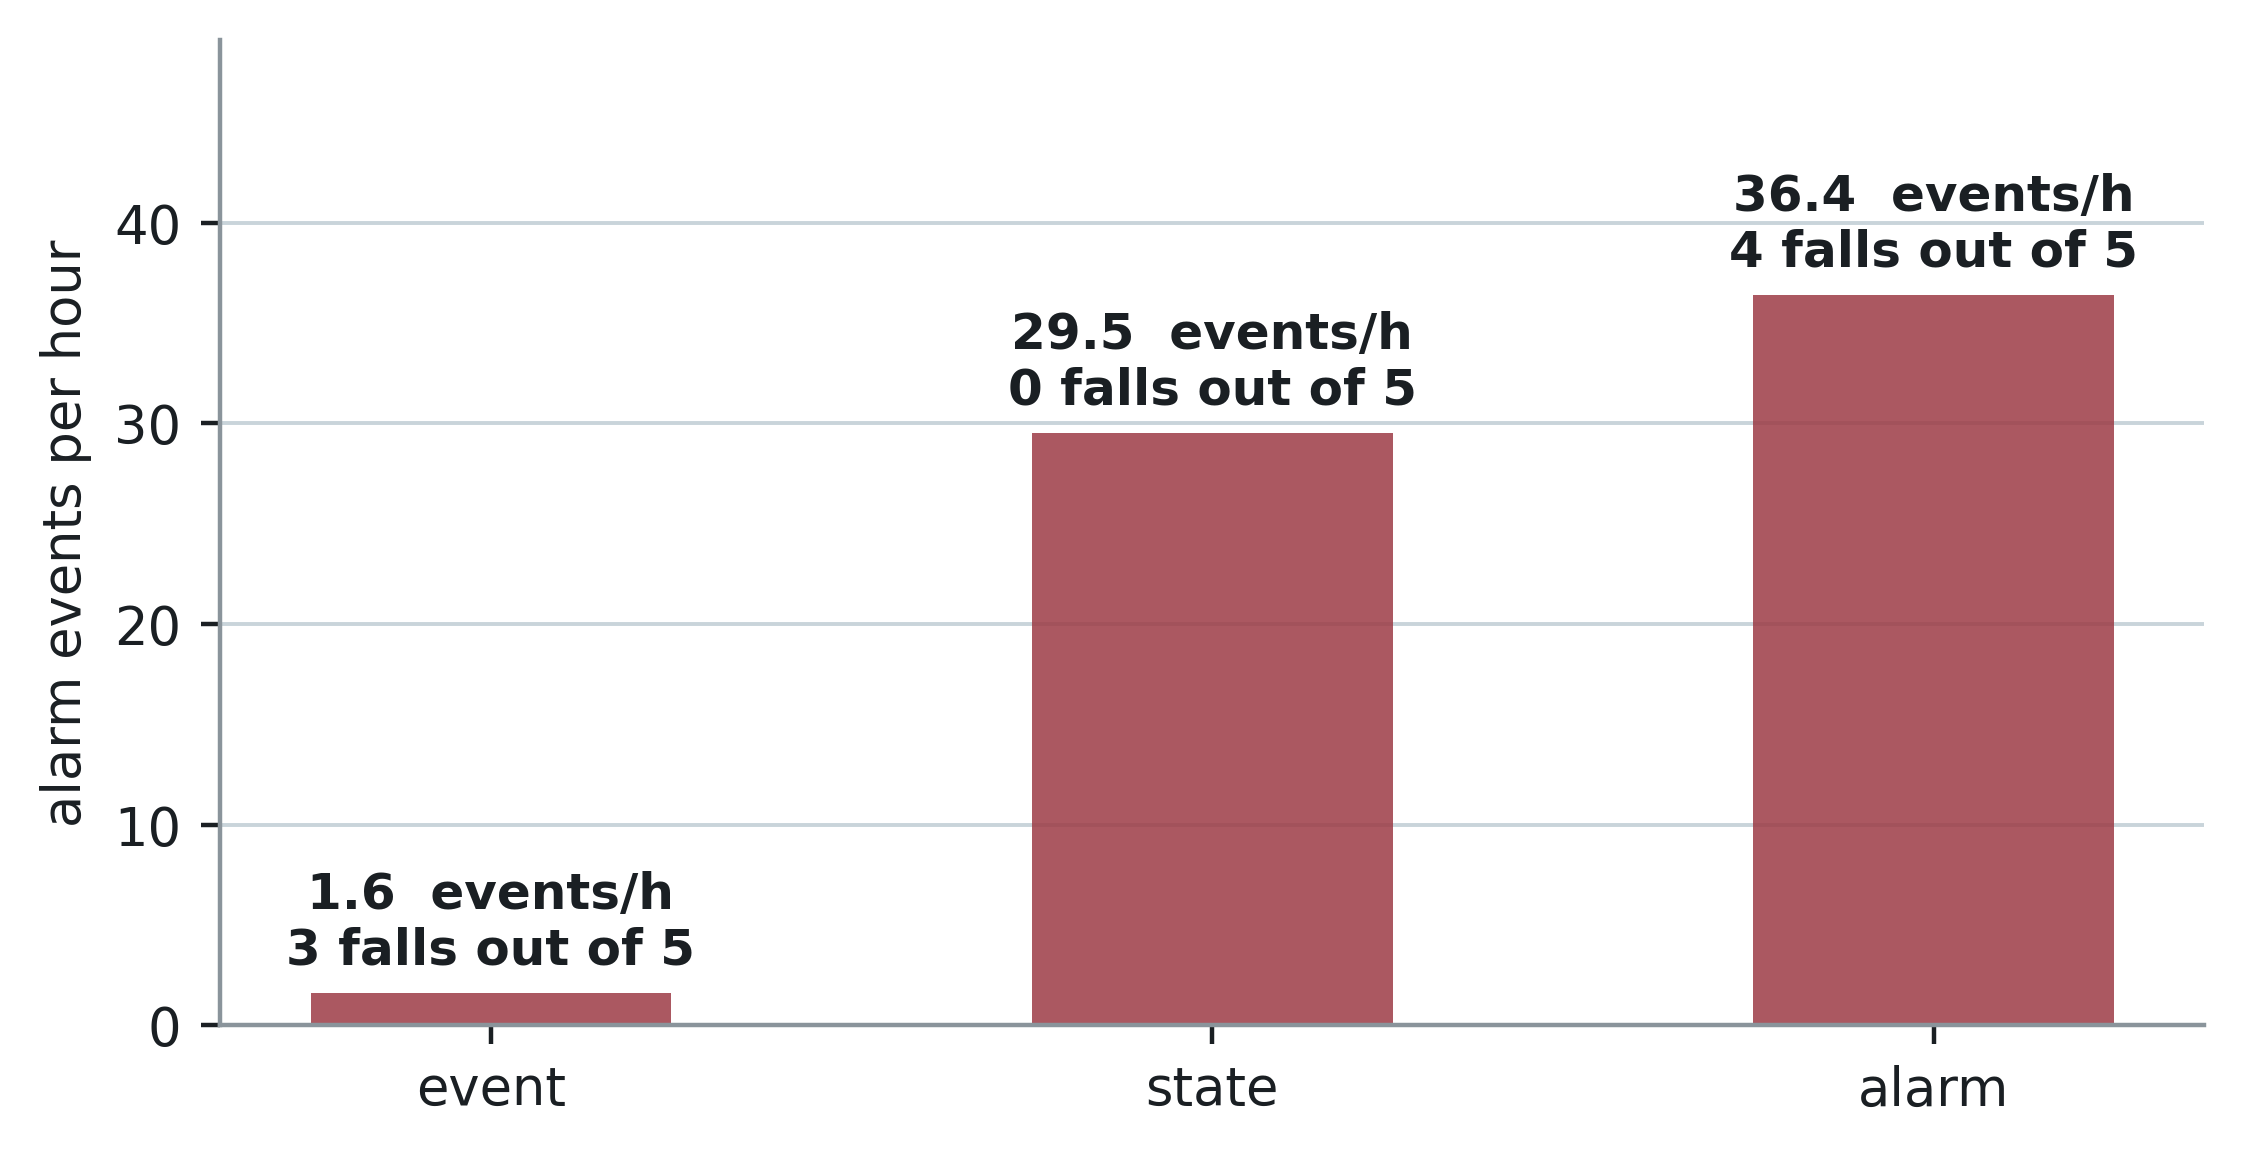
\includegraphics[width=.86\textwidth]{figure/fig_compiti_casa_en.png}
\caption{Comparison between the three definitions of the task in the domestic recordings, using the same event aggregation rule.}
\label{fig:compiti-casa}
\end{figure}

\subsection{Effect of the accumulation window}
\label{sec:finestra-k}

The integral quantities are computed over a sliding window of $K$ samples. Different values were tried while the rest of the pipeline was kept unchanged.
The laboratory results reported in Table~\ref{tab:effetto_k} come from the five-subject experiment and serve to describe the trend of the parameter.

\begin{table}[ht]
\centering
\caption{Effect of $K$ on the benchmark and in the domestic recordings.}
\label{tab:effetto_k}
\begin{tabular}{rrrrr}
\toprule
$K$ &
\textbf{$F_2$ laboratory} &
\textbf{FN} &
\textbf{Alarms/hour at home} &
\textbf{Falls} \\
\midrule
5  & $0{,}859\pm0{,}125$ & 23 & --    & -- \\
15 & $0{,}928\pm0{,}048$ & 24 & 137,6 & 4/5 \\
22 & $0{,}963\pm0{,}016$ & 9  & 17,3  & 4/5 \\
31 & $0{,}980\pm0{,}020$ & 4  & 14,0  & 4/5 \\
45 & $0{,}987\pm0{,}008$ & 3  & 17,0  & 3/5 \\
\bottomrule
\end{tabular}
\end{table}

On the benchmark, $F_2$ almost always increases as $K$ grows and reaches its maximum with $K=45$. At home, by contrast, going from $K=31$ to $K=45$ the alarms rise from 14,0 to 17,0 per hour and the falls recognised drop from 4/5 to 3/5.
The value $K=31$ was chosen partly on the basis of these domestic results. The choice is therefore not independent of the data used in the evaluation. Repeating the selection within the individual folds, nine folds out of ten choose $K=45$ and the mean $F_2$ increases by 0,026. If the laboratory result alone were used, $K=31$ would therefore not be chosen.

With $K=31$ the integral features use a longer history than the 22-sample window supplied to the classifier. The system remains causal, because only samples already observed are used and the accumulation is reset between independent recordings. $K$ does, however, represent a number of samples and not a fixed duration. At the median cadence of the archive, 31 samples correspond to about 1,72~s; across the recordings of the dataset the duration varies roughly between 1,58 and 2,15~s. On the device the misalignment is greater. At 9~fps, 31 samples correspond to about 3,4~s and, taking the classifier window into account as well, some features may depend on a total history of close to 5,8~s.

When the frequency of the board drops, the same number of samples covers an even longer interval. One solution for the future is to define $K$ as a duration and derive the number of samples from the actual frequency, instead of keeping it fixed.

\section{Failure modes and operational limitations}
\label{sec:fallimenti}
\label{sec:modi-fallire}

The domestic trials made it possible to observe some problems that do not emerge directly from the evaluation on the dataset. They concern both the representation used by the classifier and the prolonged operation of the device.

\subsection{Errors tied to the representation and to the scene}

The false positives on people lying down led us to check how far the score produced depended on the movement present in the window. The correlation measured is $+0{,}139$, therefore very low. The instantaneous derivatives moreover turned out to be sensitive to the noise of the pose and did not describe the dynamics in a stable way. From this observation the integral quantities used in configuration A3i were introduced.

A second problem concerns raised surfaces. In the negative frames with the person in a horizontal position, the median height of the hips is about $+0{,}02$ trunk lengths in the dataset and $+1{,}47$ in the domestic recordings. In the first case the person is generally close to the floor; in the second they may be lying on a bed or a sofa. This difference led to the reintroduction of $h_{\text{pav}}$ and to the use of the domestic counter-examples.

A geometric filter based on the trunk angle was also tested. With a threshold of $110^\circ$ the false positives drop from 141 to 65, but recall falls from 0,941 to 0,872 and the false negatives increase. The filter was therefore not retained in the final configuration.

\subsection{Presence of several people}

The pipeline was extended so as to keep the identity and the feature state of every person observed separate. In the only sequence available with
two people visible at the same time, made up of 291 frames, no
identity swaps were observed. The trial is, however, too short to validate multi-person tracking. UP-Fall, too, almost always contains a single person and cannot be used to check this case.

The presence of several people also increases the computational cost, because landmark estimation is carried out separately for each subject. In the trials, about 7,5~fps were measured with the room empty, 4~fps with one person and 2--3~fps with two. The reduction in frequency also changes the time interval represented by the windows. At 2--3~fps, 22 samples cover a much longer interval than the one used during training.

\subsection{Problems of continuous operation}
During one of the prolonged sessions the operating system suspended the board for about 68 minutes. The program remained active and resumed normally after the wake-up. A check between system time and monotonic time was therefore added in order to detect any interruptions.

We also observed the loss of the USB camera. In some cases the device is renumbered by the operating system, for example from \texttt{/dev/video0} to \texttt{/dev/video1}. The program may then remain active without receiving new frames. The camera is read in a separate thread and the main loop checks the time elapsed since the last frame. If it exceeds 20~s, the device is reopened. In the longest session this mechanism recovered capture in about twenty seconds; in an earlier trial the same problem had produced several minutes without images.

A further limitation concerns the computation of events per hour. Across the nine sessions considered, 1,41~hours without decisions are observed out of 14,98~total hours. Computing the rate only over the hours in which the system was actually producing decisions, the value goes from 11,1 to 12,2 events per hour, about 10\% more. The ratio between positive windows and events, 44,8, does not change, because both quantities are computed on the same decisions.

Taken together, the trials show that the pipeline can be run locally and kept active for prolonged periods, but they are not enough for the system to be regarded as validated for a real installation. The acquisitions concern only two homes and five simulated falls. Moreover, the session containing the five falls has a share of valid poses of 25,9\%, owing to sub-optimal framing. The recall values obtained in this part must therefore be read with these limitations in mind.

